\documentclass{pharmposter}
\usepackage{lipsum}
\usepackage{tikz}
\usepackage{float}

\title{BlurNet: Defense by \\Filtering the Feature Maps}
% Don't use \and with this class
\author{Ravi Raju \\ {\Large(rraju2@wisc.edu)} \\ Mikko Lipasti}

\begin{document}
	\begin{sectionbox}{Introduction}

	\begin{center}
		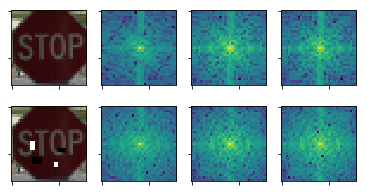
\includegraphics[scale=2.0]{regular_blur.png}
	\end{center}
	\end{sectionbox}

	\begin{sectionbox}{Background}
		\begin{center}
		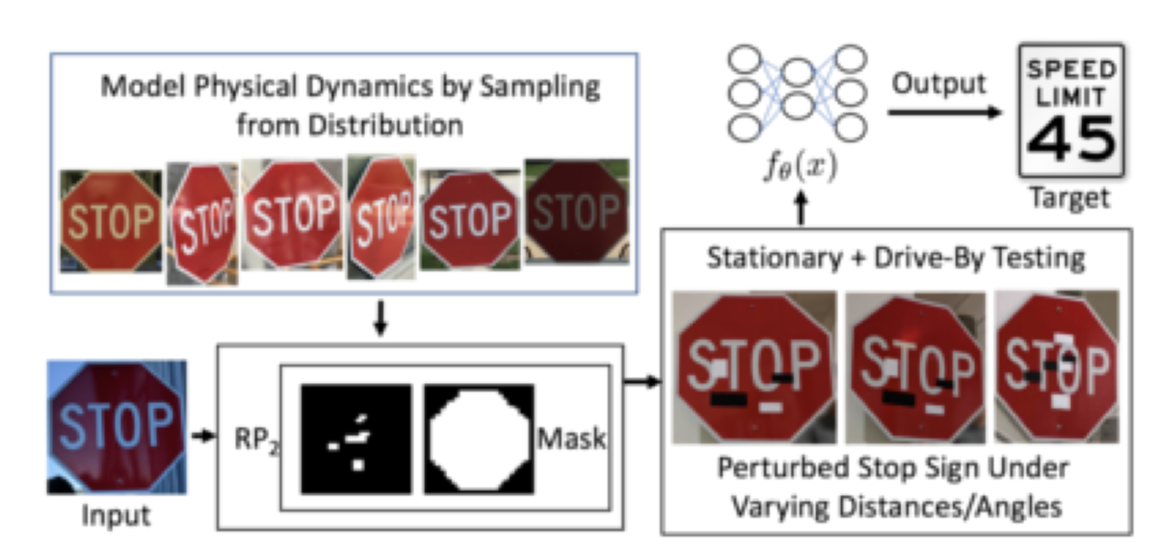
\includegraphics[scale=1.5]{RP2.png}
		\end{center}
	\end{sectionbox}

	\begin{sectionbox}{idk}
		\lipsum[2]
	\end{sectionbox}

	\begin{sectionbox}{Motivation}
		\lipsum[2]
		\begin{center}
		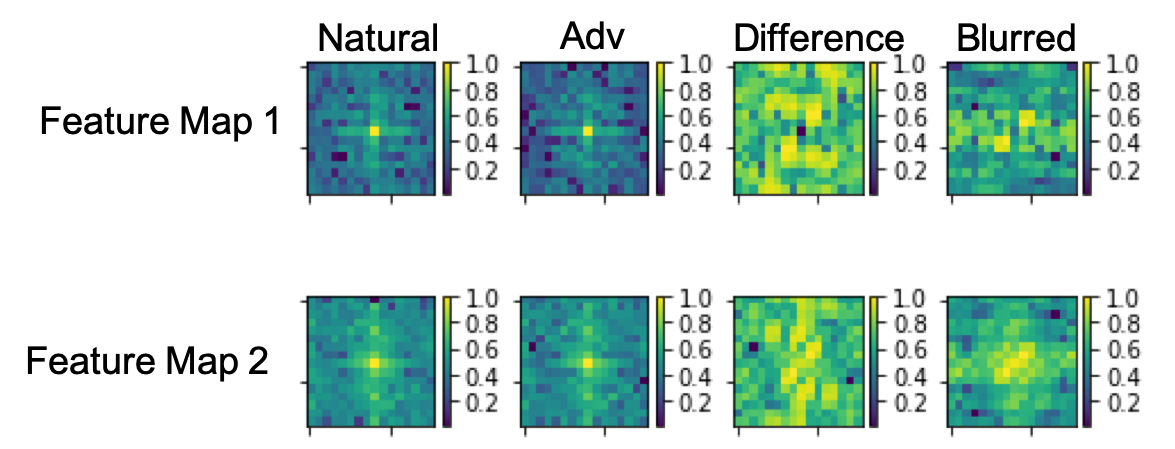
\includegraphics[scale=1.5]{fft_feat_maps_labeled.png}
		\end{center}
	\end{sectionbox}

	\begin{sectionbox}{A Figure!}
		\begin{center}
			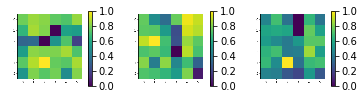
\includegraphics[scale=2.0]{higher_filters.png}
		\end{center}
	\end{sectionbox}

	\begin{sectionbox}{Results}
		\begin{table}[h!]
		  \begin{center}
		    \caption{Results from black box evaluation}
		    \label{tab:transfer}
		    \begin{tabular}{c|c|c} % <-- Alignments: 1st column left, 2nd middle and 3rd right, with vertical lines in between
		      & \textbf{Accuracy} & \textbf{Attack Success Rate}\\
		      \hline
		      Baseline & 100\% & 90\%\\
		      Input filter 3x3 & 100\% & 87.5\%\\
		      Input filter 5x5 & 100\% & 67.5\%\\
		      3x3 filter on L1 feature maps & 100\% & 65\%\\
		      5x5 filter on L1 feature maps & 87.5\% & 17.5\%\\
		    \end{tabular}
		  \end{center}
		\end{table}

		\begin{center}
		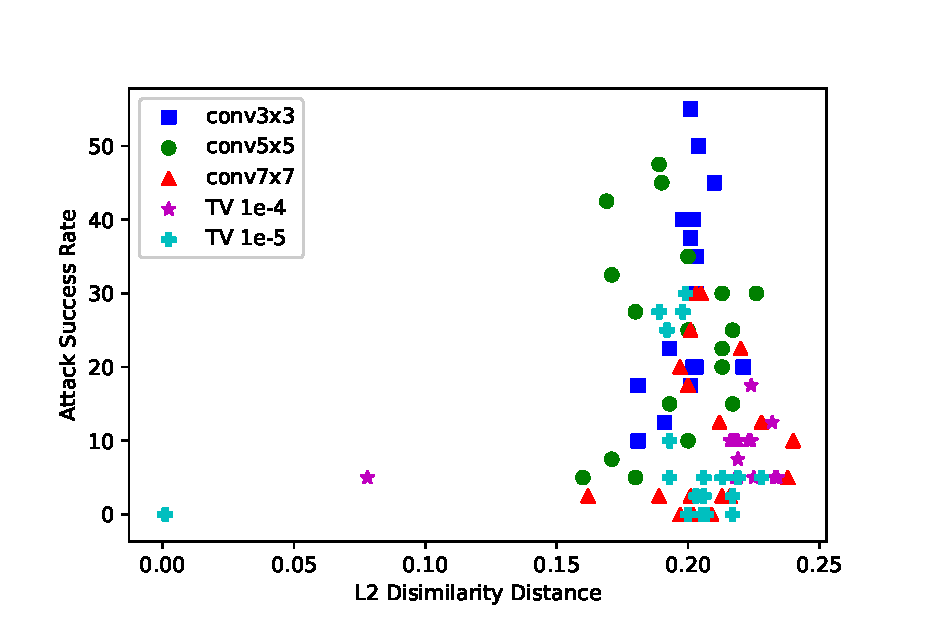
\includegraphics[scale=1.5]{L2vsAttkplot.eps}
		\end{center}
	\end{sectionbox}

	\begin{sectionbox}{Future Work}
		\lipsum[3]
	\end{sectionbox}

	\begin{sectionbox}{Related Work}
		\lipsum[7-8]
	\end{sectionbox}
\end{document}
